
\definecolor{cffff00}{RGB}{255,255,0}
\usetikzlibrary{arrows}

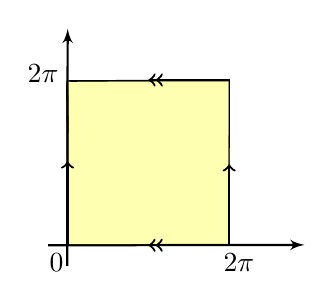
\begin{tikzpicture}[y=0.80pt, x=0.8pt,yscale=-1,scale=0.3, inner sep=0pt, outer sep=0pt]
\begin{scope}[shift={(16.51171,-222.86883)}]% layer1
  \begin{scope}[shift={(920.7302,-2377.8427)}]% g2127
    \begin{scope}[shift={(1217.3295,178.01263)}]% g1961-2
      % path1880-3
      \path[draw=black,line join=miter,line cap=butt,line width=0.800pt,-latex']
        (-2134.6966,2748.6554) -- (-1748.5202,2748.0614);

      % path1882-7
      \path[draw=black,line join=miter,line cap=butt,line width=0.800pt,-latex']
        (-2105.6782,2779.7419) -- (-2105.1084,2422.6997);

    \end{scope}
    % rect1989
    \path[shift={(5.63871,301.66294)},color=black,draw=black,fill=cffff00,opacity=0.300,line
      join=round,line cap=round,miter limit=4.00,nonzero rule,dash
      phase=16.000pt,line width=0.800pt,rounded corners=0.0000cm]
      (-893.5422,2377.1589) rectangle (-650.2519,2624.5854);

    % rect1991
    \path[shift={(5.63871,301.66294)},color=black,fill=black,line width=0.800pt]
      (-895.5773,2402.7889) .. controls (-895.0931,2439.8706) and
      (-894.8552,2476.9218) .. (-894.6665,2513.9962) .. controls
      (-894.4778,2551.0706) and (-894.3383,2588.1683) .. (-894.1753,2625.2185) ..
      controls (-889.8501,2625.2085) and (-885.5248,2625.2025) ..
      (-881.1998,2625.1925) .. controls (-842.5575,2625.1105) and
      (-804.0385,2625.1285) .. (-765.4531,2625.1585) .. controls
      (-726.8677,2625.1885) and (-688.2159,2625.2295) .. (-649.6450,2625.1925) ..
      controls (-649.6470,2623.5864) and (-649.6480,2621.9803) ..
      (-649.6500,2620.3740) .. controls (-649.6720,2600.6502) and
      (-649.6530,2580.9725) .. (-649.6133,2561.2826) .. controls
      (-649.5739,2541.5926) and (-649.5143,2521.8904) .. (-649.4559,2502.1579) ..
      controls (-649.3974,2482.4254) and (-649.3400,2462.6626) ..
      (-649.3049,2442.8918) .. controls (-649.2697,2423.1210) and
      (-649.2569,2403.3422) .. (-649.2874,2383.6180) .. controls
      (-649.2914,2381.1471) and (-649.2954,2378.6765) .. (-649.2990,2376.2062) ..
      controls (-725.6595,2376.0301) and (-801.9274,2375.9960) ..
      (-877.8829,2376.3768) .. controls (-888.7046,2375.7994) and
      (-893.7886,2376.7187) .. (-893.5329,2377.6405) .. controls
      (-893.2773,2378.5623) and (-887.7494,2379.4189) .. (-877.3298,2378.7339) ..
      controls (-801.9695,2378.1316) and (-726.3742,2377.8718) ..
      (-650.7634,2377.6706) .. controls (-650.7624,2379.6122) and
      (-650.7614,2381.5540) .. (-650.7604,2383.4958) .. controls
      (-650.7501,2402.8264) and (-650.7829,2422.2016) .. (-650.8374,2441.5592) ..
      controls (-650.8919,2460.9169) and (-650.9680,2480.2570) ..
      (-651.0445,2499.5579) .. controls (-651.1210,2518.8588) and
      (-651.1979,2538.1204) .. (-651.2537,2557.3611) .. controls
      (-651.3096,2576.6018) and (-651.3444,2595.8216) .. (-651.3370,2615.0791) ..
      controls (-651.3360,2617.8781) and (-651.3340,2620.6870) ..
      (-651.3320,2623.5052) .. controls (-688.6463,2623.5312) and
      (-727.4750,2623.6321) .. (-766.3569,2623.7446) .. controls
      (-805.2388,2623.8572) and (-844.1743,2623.9814) .. (-881.4471,2624.0545) ..
      controls (-885.3264,2624.0645) and (-889.1860,2624.0675) ..
      (-893.0273,2624.0715) .. controls (-892.9843,2587.6801) and
      (-892.7535,2552.6287) .. (-892.5065,2517.6202) .. controls
      (-892.2595,2482.6118) and (-891.9950,2447.6476) .. (-892.2515,2411.0634) ..
      controls (-892.3374,2404.0338) and (-892.6752,2393.2709) ..
      (-893.2271,2385.7558) .. controls (-893.7789,2378.2407) and
      (-894.5527,2373.9655) .. (-895.3643,2380.0575) .. controls
      (-895.7663,2386.7333) and (-895.6353,2395.2566) .. (-895.5773,2402.7889) --
      cycle;

    % text2107
    \path[shift={(5.63871,301.66294)},fill=black] (-920.45374,2665.) node[above
      right] (text2107) {$0$};

    % text2111
    \path[shift={(5.63871,301.66294)},fill=black] (-658.7821,2665.) node[above
      right] (text2111) {$2\pi$};

    % text2115
    \path[shift={(5.63871,301.66294)},fill=black] (-953.63062,2380.092) node[above
      right] (text2115) {$2\pi$};

    % path2119
    \path[shift={(5.63871,301.66294)},draw=black,line join=miter,line cap=butt,line
      width=0.800pt,->>] (-644.1132,2624.9604) -- (-771.8971,2624.9604);

    % path2121
    \path[draw=black,line join=miter,line cap=butt,line width=0.800pt,->]
      (-644.6132,2926.7484) -- (-644.6132,2804.7077);

    % path2123
    \path[draw=black,line join=miter,line cap=butt,line width=0.800pt,->>]
      (-644.1132,2677.8219) -- (-766.1539,2677.8219);

    % path2125
    \path[draw=black,line join=miter,line cap=butt,line width=0.800pt,->]
      (-887.9035,2926.7484) -- (-887.9035,2800.3626);

  \end{scope}
\end{scope}

\end{tikzpicture}

